%!TEX root=thesis.tex
\chapter{Results}

To analyze the performance of the AlphaZero algorithm for constructing pulse sequences, different sets of algorithm hyperparameters and system parameters were tested. AlphaZero was first run with no additional constraints to the tree search (i.e. the state space contains all possible sequences of pulses), and the simulated spin systems were idealized (i.e. delta-pulses and no experimental errors). Additional constraints were then added to the tree search while keeping idealized spin system simulations. Finally, experimental imperfections were introduced to the simulations.



As a preliminary consistency check, the AlphaZero algorithm was run with identical settings 10 times, and the resulting distribution of rewards during training was recorded. In figure~\ref{fig:az-consistency}, it is evident that most of the runs perform similarly, but a few significantly outperform the rest, achieving over an order of magnitude improvement in fidelity. Furthermore, most of the runs plateau after about 5000 training steps, indicating the policy network converged to a particular policy. The inconsistent performance across identical runs could be improved by further tuning the algorithm hyperparameters, such as the amount of noise added to the policy, increasing the exploration rate in the MCTS, or adjusting the relative rate of training to data collection.

\begin{figure}[H]
    \centering
    \includegraphics[width=.7\textwidth]{az-consistency.pdf}
    \caption{The mean reward ($-\log(1-\text{fidelity})$) seen during training for 10 identical runs of the AlphaZero algorithm searching for $24\tau$ sequences. The simulations included finite pulse width with no experimental errors. Most runs converge to similar mean fidelities, but a few runs have orders of magnitude better performance.}
    \label{fig:az-consistency}
\end{figure}


For the completely unconstrained search and idealized spin system simulations, AlphaZero converges to an effective
policy only for the 12-pulse sequence (figure~\ref{fig:reward_hist-no_errors-no_constraints-12}). AlphaZero tries random pulse sequences with low fidelity early in training, but quickly ``learns'' to construct pulse sequences with fidelity $\approx 1 - 10^{-8}$.

\begin{figure}[H]
    \centering
    \begin{subfigure}{.49\textwidth}
        \centering
        \includegraphics[width=\textwidth]{hists/reward_hist-no_errors-no_constraints-12.pdf}
        \caption{$12\tau$ sequence}
        \label{fig:reward_hist-no_errors-no_constraints-12}
    \end{subfigure}
    \begin{subfigure}{.49\textwidth}
        \centering
        \includegraphics[width=\textwidth]{hists/reward_hist-no_errors-no_constraints-24.pdf}
        \caption{$24\tau$ sequence}
        \label{fig:reward_hist-no_errors-no_constraints-24}
    \end{subfigure}
    \begin{subfigure}{.49\textwidth}
        \centering
        \includegraphics[width=\textwidth]{hists/reward_hist-no_errors-no_constraints-48.pdf}
        \caption{$48\tau$ sequence}
        \label{fig:reward_hist-no_errors-no_constraints-48}
    \end{subfigure}
    \caption{Distribution of rewards ($-\log(1 - \text{fidelity})$) during AlphaZero training. No constraints were applied to the tree search, and the simulated spin systems were idealized.}
    \label{fig:reward_hist-no_errors-no_constraints}
\end{figure}

However, for longer pulse sequences with 24 or 48 actions, unconstrained search is unable to converge to similarly effective policies as for shorter sequences. For the 24-pulse sequence (figure~\ref{fig:reward_hist-no_errors-no_constraints-24}), the policy after 2000 training steps constructs pulse sequences with fidelity $\approx 1 - 10^{-6}$, about two orders of magnitude worse than for the 12-pulse sequence.
And for the 48-pulse sequence (figure~\ref{fig:reward_hist-no_errors-no_constraints-24}), the policy constructs pulse sequences with even lower fidelities. Even after 8000 training steps, the policy still constructs pulse sequences with fidelity $\approx 0$ over $30\%$ of the time.

The worsening performance as the pulse sequence length increases is understandable. For an $n$-pulse sequence with $a$ possible actions, there are $a^n$ possible pulse sequences, and $\frac{a^{n+1} - 1}{a-1}$ possible states%
\footnote{
This can be seen by counting how many subsequences of length $k$ there are ($a^k$), and adding these for $k = 1, \dots, n$.
}.
If $n=12$, then there are over 244 million pulse sequences and over 300 million states.
But for $n=24$, then the number of pulse sequences jumps to $6 \times 10^{16}$, and for $n=48$ there are $3.6 \times 10^{33}$. Because AlphaZero begins training \emph{tabula rasa}, none of the states in the astronomically large state space are preferred by the agent, so it begins with a purely random search.
Furthermore, rewards are only received once an \emph{entire pulse sequence} has been constructed. The sparse reward signal (which is the sole driver of learning in RL algorithms) therefore makes it difficult for the agent to associate actions with rewards and learn an effective policy.
This is known as the ``credit assignment problem'' and is an active area of research both in theoretical and applied RL (\cite{arumugam2021informationtheoretic}).

For example, suppose you needed to pass a test with $100$ questions, and could re-take the test as many times as you want. It would take many more tries to pass if the only feedback you received was your overall score on the test, as opposed to your score on each question.

There is not an immediately obvious way to provide additional rewards to the agent during training\footnote{
From an experimental perspective, we only care about the fidelity of the pulse sequence overall, not at intermediate times.
},
but there are ways to constrain AlphaZero's tree search to only consider subsets of the state space.
As described in section~\ref{sec:AHT-constraints}, the lowest-order term in the average Hamiltonian can be set to the desired Hamiltonian by
requiring that the toggling frame spend equal durations in different orientations.
To decouple all interactions, the toggling frame must spend equal time along each axis (i.e. $I_z$ must be toggled to $\pm I_x, \pm I_y, \pm I_z$ for equal times).
By adding this constraint to the tree search, all pulse sequences at least have the correct average Hamiltonian to lowest order. This does not address the cyclic requirement for those pulse sequences (i.e. the toggling frame coincide with the lab frame at the end of the pulse sequence), the higher-order terms in the average Hamiltonian, nor experimental imperfections.

Figure~\ref{fig:reward_hist-no_errors-AHT0} shows the distributions of pulse sequence fidelities for the $12\tau, 24\tau$, and $48\tau$ sequences during training. Despite restricting the state space in a way that should guarantee higher fidelities, the fidelities are actually lower for the $12\tau$ and $24\tau$ sequences, and are comparable for the $48\tau$ sequence. These discrepancies are likely due to the inherent randomness of the algorithm (as seen in figure~\ref{fig:az-consistency}), but more careful analysis is needed to understand the observed differences.

\begin{figure}[H]
    \centering
    \begin{subfigure}{.49\textwidth}
        \centering
        \includegraphics[width=\textwidth]{hists/reward_hist-no_errors-AHT0-12.pdf}
        \caption{$12\tau$ sequence}
        \label{fig:reward_hist-no_errors-AHT0-12}
    \end{subfigure}
    \begin{subfigure}{.49\textwidth}
        \centering
        \includegraphics[width=\textwidth]{hists/reward_hist-no_errors-AHT0-24.pdf}
        \caption{$24\tau$ sequence}
        \label{fig:reward_hist-no_errors-AHT0-24}
    \end{subfigure}
    \begin{subfigure}{.49\textwidth}
        \centering
        \includegraphics[width=\textwidth]{hists/reward_hist-no_errors-AHT0-48.pdf}
        \caption{$48\tau$ sequence}
        \label{fig:reward_hist-no_errors-AHT0-48}
    \end{subfigure}
    \caption{Distribution of rewards ($-\log(1 - \text{fidelity})$) during AlphaZero training. Lowest-order AHT constraints were applied to the tree search, and the simulated spin systems were idealized.}
    \label{fig:reward_hist-no_errors-AHT0}
\end{figure}


Because the lowest-order average Hamiltonian constraint didn't clearly improve performance, an even stronger constraint was added to the tree search to further restrict the state space: to decouple interactions to lowest order every $6\tau$, instead of decoupling interactions for the pulse sequence overall.
There are $200$ sequences of length $6\tau$ that will decouple all interactions to lowest order, significantly fewer than $5^6 = 15625$ possible sequences without any constraints. The resulting fidelities (figure~\ref{fig:reward_hist-no_errors-6tau}) are significantly higher for the $24\tau$ and $48\tau$ sequences during training, comparable to the shorter $12\tau$ sequence.

\begin{figure}[H]
    \centering
    \begin{subfigure}{.49\textwidth}
        \centering
        \includegraphics[width=\textwidth]{hists/reward_hist-no_errors-6tau-12.pdf}
        \caption{$12\tau$ sequence}
        \label{fig:reward_hist-no_errors-6tau-12}
    \end{subfigure}
    \begin{subfigure}{.49\textwidth}
        \centering
        \includegraphics[width=\textwidth]{hists/reward_hist-no_errors-6tau-24.pdf}
        \caption{$24\tau$ sequence}
        \label{fig:reward_hist-no_errors-6tau-24}
    \end{subfigure}
    \begin{subfigure}{.49\textwidth}
        \centering
        \includegraphics[width=\textwidth]{hists/reward_hist-no_errors-6tau-48.pdf}
        \caption{$48\tau$ sequence}
        \label{fig:reward_hist-no_errors-6tau-48}
    \end{subfigure}
    \caption{Distribution of rewards ($-\log(1 - \text{fidelity})$) during AlphaZero training. Lowest-order AHT constraints and refocusing all interactions every $6\tau$ were applied to the tree search, and the simulated spin systems were idealized.}
    \label{fig:reward_hist-no_errors-6tau}
\end{figure}

The $6\tau$ refocusing constraint, while empirically beneficial for the AlphaZero tree search, raises some questions. By introducing this constraint, is the algorithm excluding high-fidelity pulse sequences that do not follow this constraint? The CORY48 pulse sequence in fact does not refocus \emph{all} interactions to lowest order until the end of the pulse sequence, and its fidelity is much higher than any pulse sequence found using AlphaZero. Instead, it decouples dipolar interactions every $9\tau$, which is a more relaxed constraint.

% TODO include figure showing refocusing interactions
% TODO...

During training, pulse sequences with fidelity above a given threshold are recorded, and the highest-fidelity pulse sequence is chosen as a ``candidate'' for further evaluation (it would be impractical to evaluate each of the thousands of pulse sequences constructed by AlphaZero).
The AlphaZero algorithm was originally designed to play board games, where the trained policy function defined on the entire state space is more important than the specific sequence of moves played in training games. In contrast, for designing pulse sequences, the final policy is less important than identifying a single pulse sequence with high fidelity and robustness to errors. The policy is only a tool for exploring the state space for high-fidelity pulse sequences.



\section{Robustness Evaluation}

Although it is straightforward to simulate spin systems under ideal conditions without any experimental imperfections, this never happens in reality. Therefore, it is important to consider how the pulse sequences perform in the presence of errors and determine their robustness.
The errors considered below include pulse rotation errors, phase transient errors, and resonant offset errors.
% TODO include delay time too???

Pulse rotation errors, either under- or over-rotating the spins, are common in NMR and electron spin resonance (ESR) systems due to limited precision in both the rf-field strength and the pulse width $t_p$. If the pulse strength or duration is too high (or too low), then the toggling frame will be rotated greater (or less) than $\pi/2$ and the average Hamiltonian will not necessarily match the target Hamiltonian. See figure~\ref{fig:rotation-error} for a visual depiction of rotation errors for a single spin.

\begin{figure}[H]
    \centering
    

\tikzset{every picture/.style={line width=0.75pt}} %set default line width to 0.75pt

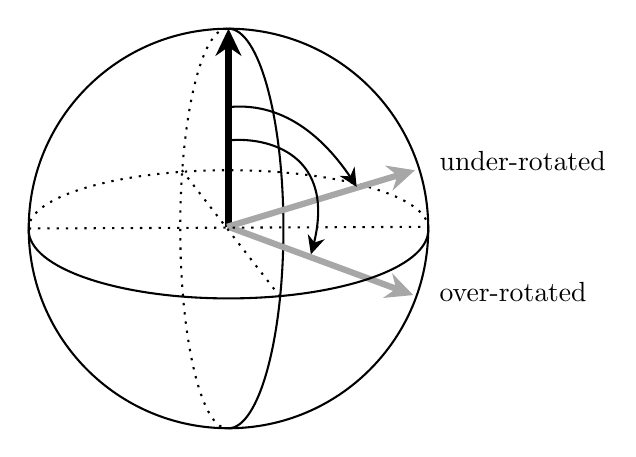
\begin{tikzpicture}[x=0.75pt,y=0.75pt,yscale=-1,xscale=1]
%uncomment if require: \path (0,300); %set diagram left start at 0, and has height of 300

%Shape: Arc [id:dp782370095502481]
\draw  [draw opacity=0][dash pattern={on 0.84pt off 2.51pt}] (212.5,116.75) .. controls (212.5,101.25) and (169.41,88.68) .. (116.25,88.68) .. controls (63.09,88.68) and (20,101.25) .. (20,116.75) .. controls (20,116.75) and (20,116.75) .. (20,116.75) -- (116.25,116.75) -- cycle ; \draw  [dash pattern={on 0.84pt off 2.51pt}] (212.5,116.75) .. controls (212.5,101.25) and (169.41,88.68) .. (116.25,88.68) .. controls (63.09,88.68) and (20,101.25) .. (20,116.75) .. controls (20,116.75) and (20,116.75) .. (20,116.75) ;
%Shape: Circle [id:dp3404154288852026]
\draw   (20,116.75) .. controls (20,63.59) and (63.09,20.5) .. (116.25,20.5) .. controls (169.41,20.5) and (212.5,63.59) .. (212.5,116.75) .. controls (212.5,169.91) and (169.41,213) .. (116.25,213) .. controls (63.09,213) and (20,169.91) .. (20,116.75) -- cycle ;
%Straight Lines [id:da667885384509429]
\draw [line width=2.25]    (116.25,115.95) -- (116.25,25.5) ;
\draw [shift={(116.25,20.5)}, rotate = 450] [fill={rgb, 255:red, 0; green, 0; blue, 0 }  ][line width=0.08]  [draw opacity=0] (13.22,-6.35) -- (0,0) -- (13.22,6.35) -- (8.78,0) -- cycle    ;
%Shape: Arc [id:dp19644604622327155]
\draw  [draw opacity=0] (116.25,20.5) .. controls (116.25,20.5) and (116.25,20.5) .. (116.25,20.5) .. controls (116.25,20.5) and (116.25,20.5) .. (116.25,20.5) .. controls (130.87,20.5) and (142.72,63.59) .. (142.72,116.75) .. controls (142.72,169.91) and (130.87,213) .. (116.25,213) -- (116.25,116.75) -- cycle ; \draw   (116.25,20.5) .. controls (116.25,20.5) and (116.25,20.5) .. (116.25,20.5) .. controls (116.25,20.5) and (116.25,20.5) .. (116.25,20.5) .. controls (130.87,20.5) and (142.72,63.59) .. (142.72,116.75) .. controls (142.72,169.91) and (130.87,213) .. (116.25,213) ;
%Shape: Arc [id:dp34236219446094807]
\draw  [draw opacity=0][dash pattern={on 0.84pt off 2.51pt}] (115.6,20.5) .. controls (115.6,20.5) and (115.6,20.5) .. (115.6,20.5) .. controls (103.13,20.5) and (93.01,63.59) .. (93.01,116.75) .. controls (93.01,169.91) and (103.13,213) .. (115.6,213) -- (115.6,116.75) -- cycle ; \draw  [dash pattern={on 0.84pt off 2.51pt}] (115.6,20.5) .. controls (115.6,20.5) and (115.6,20.5) .. (115.6,20.5) .. controls (103.13,20.5) and (93.01,63.59) .. (93.01,116.75) .. controls (93.01,169.91) and (103.13,213) .. (115.6,213) ;

%Straight Lines [id:da42656322211334885]
\draw [color={rgb, 255:red, 167; green, 167; blue, 167 }  ,draw opacity=1 ][line width=2.25]    (116.25,115.95) -- (200.59,147.1) ;
\draw [shift={(205.28,148.83)}, rotate = 200.27] [fill={rgb, 255:red, 167; green, 167; blue, 167 }  ,fill opacity=1 ][line width=0.08]  [draw opacity=0] (13.22,-6.35) -- (0,0) -- (13.22,6.35) -- (8.78,0) -- cycle    ;
%Straight Lines [id:da7850995960487122]
\draw [color={rgb, 255:red, 167; green, 167; blue, 167 }  ,draw opacity=1 ][line width=2.25]    (115.6,115.95) -- (201.3,90.12) ;
\draw [shift={(206.08,88.68)}, rotate = 523.23] [fill={rgb, 255:red, 167; green, 167; blue, 167 }  ,fill opacity=1 ][line width=0.08]  [draw opacity=0] (13.22,-6.35) -- (0,0) -- (13.22,6.35) -- (8.78,0) -- cycle    ;
%Straight Lines [id:da4695507768944873]
\draw  [dash pattern={on 0.84pt off 2.51pt}]  (93.79,88.68) -- (141.11,149.64) ;
%Straight Lines [id:da7792399094821125]
\draw  [dash pattern={on 0.84pt off 2.51pt}]  (20,116.75) -- (212.5,115.95) ;
%Curve Lines [id:da1883472442634171]
\draw    (117.05,58.2) .. controls (144,55.89) and (163.56,74.28) .. (176.44,94.2) ;
\draw [shift={(178.01,96.7)}, rotate = 238.39] [fill={rgb, 255:red, 0; green, 0; blue, 0 }  ][line width=0.08]  [draw opacity=0] (8.93,-4.29) -- (0,0) -- (8.93,4.29) -- (5.93,0) -- cycle    ;
%Curve Lines [id:da04261734583163235]
\draw    (117.05,74.24) .. controls (134.34,72.67) and (169.36,80.34) .. (156.78,126.32) ;
\draw [shift={(155.95,129.18)}, rotate = 287] [fill={rgb, 255:red, 0; green, 0; blue, 0 }  ][line width=0.08]  [draw opacity=0] (8.93,-4.29) -- (0,0) -- (8.93,4.29) -- (5.93,0) -- cycle    ;
%Shape: Arc [id:dp9372143530929324]
\draw  [draw opacity=0] (212.5,117.55) .. controls (212.5,117.55) and (212.5,117.55) .. (212.5,117.55) .. controls (212.5,117.55) and (212.5,117.55) .. (212.5,117.55) .. controls (212.5,135.71) and (169.41,150.44) .. (116.25,150.44) .. controls (63.09,150.44) and (20,135.71) .. (20,117.55) -- (116.25,117.55) -- cycle ; \draw   (212.5,117.55) .. controls (212.5,117.55) and (212.5,117.55) .. (212.5,117.55) .. controls (212.5,117.55) and (212.5,117.55) .. (212.5,117.55) .. controls (212.5,135.71) and (169.41,150.44) .. (116.25,150.44) .. controls (63.09,150.44) and (20,135.71) .. (20,117.55) ;

% Text Node
\draw (216.48,77.86) node [anchor=north west][inner sep=0.75pt]   [align=left] {under-rotated};
% Text Node
\draw (216.48,141.23) node [anchor=north west][inner sep=0.75pt]   [align=left] {over-rotated};


\end{tikzpicture}

    \caption{Pulse rotation errors for a single spin.}
    \label{fig:rotation-error}
\end{figure}

Phase transient errors are another pulse-related error that are present in experimental systems. When applying a pulse, the non-zero impedance in the circuit will induce small additional pulses in quadrature to the intended pulse when the rf field rises and falls. For example, applying an $X$ pulse will also apply slight rotations about the $y$ axis when the $B_X$ field rises and falls. See figure~\ref{fig:phase_transients} for an ideal pulse compared to a pulse with phase transients. To simulate phase transient errors, each of the $X, Y, \overline{X}$, and $\overline{Y}$ actions were modified to include slight rotations along $y, -x, -y$, and $x$ immediately before and after the pulse. The rotation angle was parameterized as a fraction of $\pi/2$.

\begin{figure}[H]
    \centering
    \includegraphics[width=.7\textwidth]{phase_transients_viz.png}
    \caption{
    An ideal pulse (a) compared to a pulse with phase transients (b). Illustration from \cite{1976ii}.
    }
    \label{fig:phase_transients}
\end{figure}

Finally, resonance offset errors occur when the rf field is not matched to the Larmor frequency of the spins. The rotating frame therefore does not rotate \emph{precisely} with the spins, but at an offset frequency.

The highest-fidelity pulse sequences from the $12\tau, 24\tau$, and $48\tau$ sequence searches\footnote{
See the appendix for an explicit presentation of these pulse sequences.
} with AHT and $6\tau$ refocusing constraints were evaluated for robustness against the experimental imperfections introduced above. To compare each of the different-length sequences on the same footing, each pulse sequence was repeated over a total duration of $288\tau$. That is, the $12\tau$ sequence was repeated $24$ times, the $24\tau$ sequence was repeated $12$ times, the $48\tau$ repeated $6$ times, and CORY48 (a $72\tau$ sequence) repeated $4$ times.
% TODO actually put pulse sequences in appendix!!!
% TODO explain evaluation, the whole 288tau thing...



For small rotation errors ($<1\%$ of a $\pi/2$-pulse) the fidelity for all pulse sequences declines dramatically (see figure~\ref{fig:rot_errors-no_errors}).
This is not entirely unexpected however: the spin systems during training were idealized, so no errors of any kind were included. As a result, there was no reward signal for constructing \emph{robust} pulse sequences, only pulse sequences that did well under ideal conditions.





\begin{figure}[H]
    \centering
    \includegraphics[width=.7\textwidth]{robustness/rot_errors-no_errors.pdf}
    \caption{Robustness against rotation errors, relative to a $\pi/2$-pulse. Training simulations included no errors, and evaluation simulations included only rotation errors.
    The pulse sequences identified using AlphaZero have very poor robustness to rotation errors, while the CORY48 sequence (which was designed using AHT to be robust to such errors) has high fidelity for a much broader range of rotation errors.
    }
    \label{fig:rot_errors-no_errors}
\end{figure}

Similarly, the pulse sequences are much less robust to phase transient error (figure~\ref{fig:phase_transients-no_errors}), or
resonance offset error (figure~\ref{fig:offset_errors-no_errors}). Interestingly, the $12\tau$ sequence seems to be highly robust to phase transient error, but the fidelity is comparably worse overall.
% or increasing th delay $\tau$ between pulses (\ref{fig:tau_delay-no_errors}).


\begin{figure}[H]
    \centering
    \includegraphics[width=.7\textwidth]{robustness/phase_transients-no_errors.pdf}
    \caption{Robustness against phase transient errors, where the quadrature rotations are relative to a $\pi/2$-pulse.
    Training simulations included no errors, and evaluation simulations included only rotation errors.
    }
    \label{fig:phase_transients-no_errors}
\end{figure}


\begin{figure}[H]
    \centering
    \includegraphics[width=.7\textwidth]{robustness/offset_errors-no_errors.pdf}
    \caption{Robustness against resonant offset error, relative to the chemical shift strength.
    Training simulations included no errors, and evaluation simulations included only rotation errors.
    }
    \label{fig:offset_errors-no_errors}
\end{figure}

% \begin{figure}[H]
%     \centering
%     \includegraphics[width=.7\textwidth]{robustness/tau_delay-no_errors.pdf}
%     \caption{Robustness against longer $\tau$ delays between pulses.
%     }
%     \label{fig:tau_delay-no_errors}
% \end{figure}


To search for \emph{robust} pulse sequences, errors were intentionally introduced into the spin systems during training. First, only rotation errors were included by sampling a random rotation error $\epsilon_r \sim \mathcal{N}(\mu=0, \sigma=.01)$ for each spin system during training. Then instead of having perfect $\pi/2$-pulses, all pulses in a particular spin system rotate the spins by $\frac{\pi}{2}(1+\epsilon_r)$. The resulting pulse sequences were significantly more robust to rotation errors (figure~\ref{fig:rot_errors-rot_errors})
compared to training without any errors (figure~\ref{fig:rot_errors-no_errors}).

\begin{figure}[H]
    \centering
    \includegraphics[width=.7\textwidth]{robustness/rot_errors-rot_errors.pdf}
    \caption{Robustness against rotation errors, relative to a $\pi/2$-pulse.
    Training simulations included only rotation errors, and evaluation simulations included only rotation errors.
    The pulse sequences identified from training with rotation errors have improved robustness to rotation errors, as compared with training in the absence of rotation errors.
    }
    \label{fig:rot_errors-rot_errors}
\end{figure}


Finally, the AlphaZero algorithm was run with multiple experimental imperfections: rotation error $\epsilon_r \sim \mathcal{N}(0, .01)$, phase transient error $\epsilon_{pt} \sim \mathcal{N}(0, 10^{-4})$, and resonance offset error $\epsilon_o \sim \mathcal{N}(0, 10^1)$.
The policy function was rewarded for high-fidelity pulse sequences in the presence of those errors, and consequently should identify pulse subsequences robust to multiple errors. For a range of rotation, phase transient, and resonance offset error (figures~\ref{fig:rot_errors-all_errors} to~\ref{fig:offset_errors-all_errors}), the pulse sequences from training \emph{with} simulated errors are more robust than those from training with no errors.

\begin{figure}[H]
    \centering
    \includegraphics[width=.7\textwidth]{robustness/rot_errors-all_errors.pdf}
    \caption{
    Robustness against pulse rotation errors.
    Training simulations included rotation, phase transient, and resonance offset errors (``all errors''), and evaluation simulations included all errors.
    % The $12\tau, 24\tau$, and $48\tau$ pulse sequences were identified during training with rotation, phase transient, and resonance offset errors.
    }
    \label{fig:rot_errors-all_errors}
\end{figure}

\begin{figure}[H]
    \centering
    \includegraphics[width=.7\textwidth]{robustness/phase_transients-all_errors.pdf}
    \caption{
    Robustness against phase transient errors, where the quadrature rotations are relative to a $\pi/2$-pulse.
    Training simulations included rotation, phase transient, and resonance offset errors (``all errors''), and evaluation simulations included all errors.
    % The $12\tau, 24\tau$, and $48\tau$ pulse sequences were identified during training with rotation, phase transient, and resonance offset errors.
    }
    \label{fig:phase_transients-all_errors}
\end{figure}

\begin{figure}[H]
    \centering
    \includegraphics[width=.7\textwidth]{robustness/offset_errors-all_errors.pdf}
    \caption{
    Robustness against resonance offset errors, relative to chemical shift strength.
    Training simulations included rotation, phase transient, and resonance offset errors (``all errors''), and evaluation simulations included all errors.
    % The $12\tau, 24\tau$, and $48\tau$ pulse sequences were identified during training with rotation, phase transient, and resonance offset errors.
    }
    \label{fig:offset_errors-all_errors}
\end{figure}

Despite the improved robustness by including errors in training, the resulting pulse sequences still have significantly lower rewards (and thus lower fidelity) than the CORY48 pulse sequence in simulated spin systems. This holds true across different possible errors and at every magnitude of error tested. In short, the reinforcement learning approach tried in this work is not as effective as the AHT-based analytical process used to design CORY48.



\section{Experimental Validation}\label{sec:experimental}

% TODO
% explain which sequence is tested
In addition to computational simulations, the best-performing $48\tau$ pulse sequence was tested against the CORY48 pulse sequence in a solid-state NMR spectrometer.
% TODO find out the magnet specs, bruker magnet _._T
An adamantane sample was used.
% TODO find out/look up sample specs, e.g. dipolar strength is ___, CS is ___
% the CORY48 paper has stats on adamantane

While the fidelity of a unitary matrix is straightforward to calculate in simulation, measuring the fidelity in experiment is much more difficult, as it would require evaluation on a complete basis of states (i.e. quantum process tomography).
% TODO cite above
Instead, the fidelity is qualitatively approximated by the average correlation $C_\text{avg}$ (\cite{peng2021deep})
\[
C_\text{avg} = (C_{XX} C_{YY} C_{ZZ})^{1/3}
\]
where the correlation function $C_{XX}(t)$ is the expected signal from initializing the state along $X$ and measuring magnetization along $X$.
% $C_{YY}(t)$ and $C_{ZZ}(t)$ are defined similarly.

\begin{figure}[H]
    \centering
    \includegraphics[width=.7\textwidth]{decay_plot_2.pdf}
    \caption{The average correlation in an adamantane sample for the $48\tau$-pulse sequence identified using AlphaZero with all errors in training, and for the CORY48 pulse sequence.}
    \label{fig:decay_plot}
\end{figure}

The experimental correlation functions (figure~\ref{fig:decay_plot}) further support the computational results: the RL-based $48\tau$ pulse sequence does decouple interactions, but not as effectively as the CORY48 pulse sequence.
